\newcommand{\upcite}[1]{\textsuperscript{\textsuperscript{\cite{#1}}}}
\chapter{概论}
\section{神经元重建的意义}

原始神经元图像信息的神经元追踪和数字重建是神经科学界热门方向。神经元的形态反应出它的功能,相同功能的神经元通常具有类似的功能。神经科学家通过结构脑图谱的重建,可以反推大脑是如何运作,对理解智慧的产生有重要的帮助。十九世纪以来,神经科学家们开始推测记忆,甚至个性与智力都储存大脑神经元之间的连接里。图 \ref{worm} 展示了秀丽隐杆线虫的神经结构的神经结构,图中每一个节点均代表一个神经元,每一条线代表一个连接。它仅仅由 300 个神经元组成,之间的连接也仅有 7000 个。

\begin{figure}
\centering
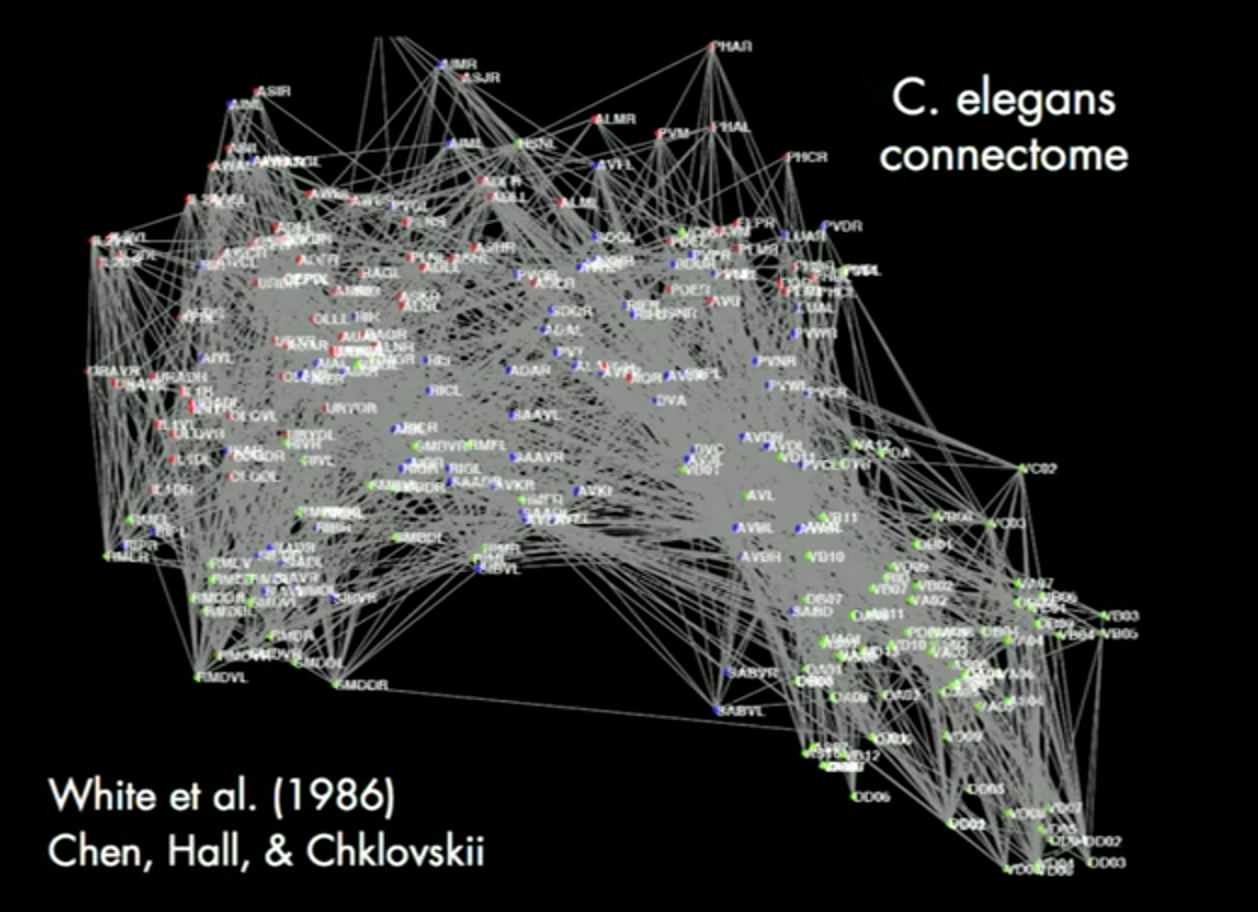
\includegraphics[width=108mm]{images/worm}
\caption{秀丽隐杆线虫的神经结构}
\label{worm}
\end{figure}

White, John G 与 Southgate 等人在 1986 年时已经 利用一系列局部原始电子显微照片对秀丽隐杆线虫的神经系统的进行了完整重建\upcite{white1986structure}。经过了 30 多年的发展,Yunkyu Sohn,Myung-Kyu Choi 与 Yong-Yeol Ahn 等人于 2011 年利用基于模块化的群态检测算法发现秀丽隐杆线虫中有 5 个解剖簇及其对应的实验可识别功能电路,进一步揭示了生物电路如何产生更高阶的复杂行为\upcite{varshney2011structural}。即使如此,由于神经网络复杂的拓扑结构,神经科学家们仍旧未能充分探索通过突触交织的神经网络结构。而人类大脑由一千亿个神经元组成,神经元之间的连接的数量又是神经元数量的一万倍,比秀丽隐杆线虫的神经结构要复杂的多。设计并实现出自动神经元重建算法便成了探索神经结构的重要步骤之一。

Druckmann, Shaul 与 Feng 等人开发的神经元重建算法提供了准确的中线,直径,表面,体积和分支点位置,支持沿着神经元表面分析标记过的分子分布,还可以直接导出到建模软件。图 \ref{Druckmann} 展示了这种神经元重建算法的样例结果。Brown, Kerry M 与 Barrionuevo 等人收集了来自不同动物,脑区,神经元类型和可视化方法的六个数据集,为自动化软件所需的测试提供了基准,提高了重建的质量,同时最大限度地减少了人工的参与,极大的促进了神经元重建领域的发展\upcite{brown2011diadem}。

\begin{figure}
\centering
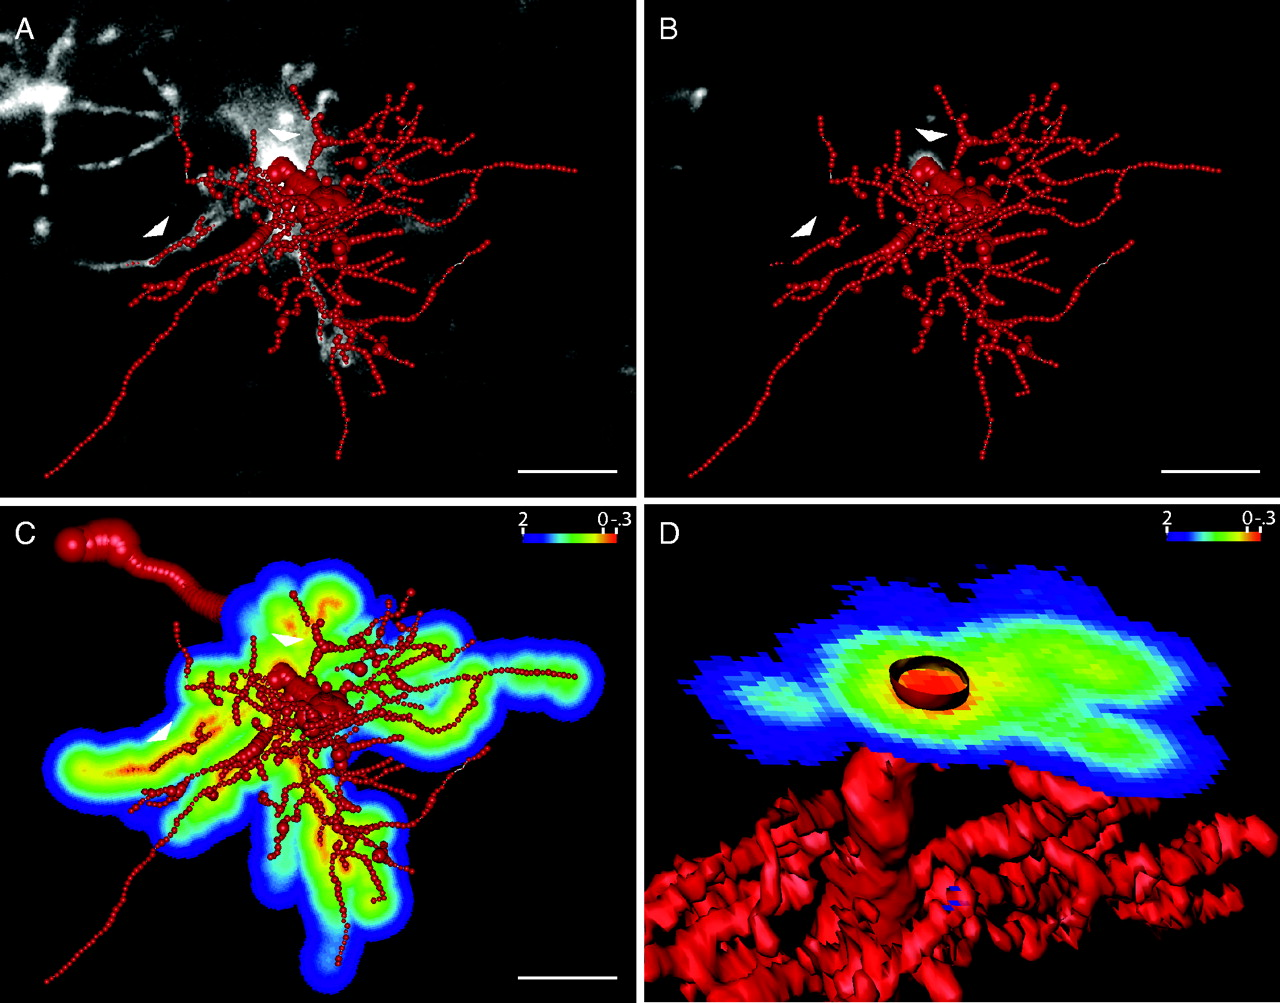
\includegraphics[width=108mm]{images/Druckmann}
\caption{Druckmann 等人的神经元重建算法的样例结果}
\label{Druckmann}
\end{figure}
